\chapter{Methodology}\label{cha:method}

\section{Data}\label{sec:dataset}
The results presented in Chapter~\ref{cha:results} are trained on data sourced from the Norwegian Asthma and Allergy Association, who have, since 1980, tracked the amount of air born pollen in Norway.
Pollen is collected with traps where air is continually sucked though a small slit and is redirected over an adhesive strip.
The strip is moved across the slit, exposing different sections throughout the day.
Pollen grains and other air born particulates adhere to the strip, which is then analyzed under a microscope.
Only pollen grains from a subset of species are actively tracked.

\begin{figure}[htbp]
  \centering
  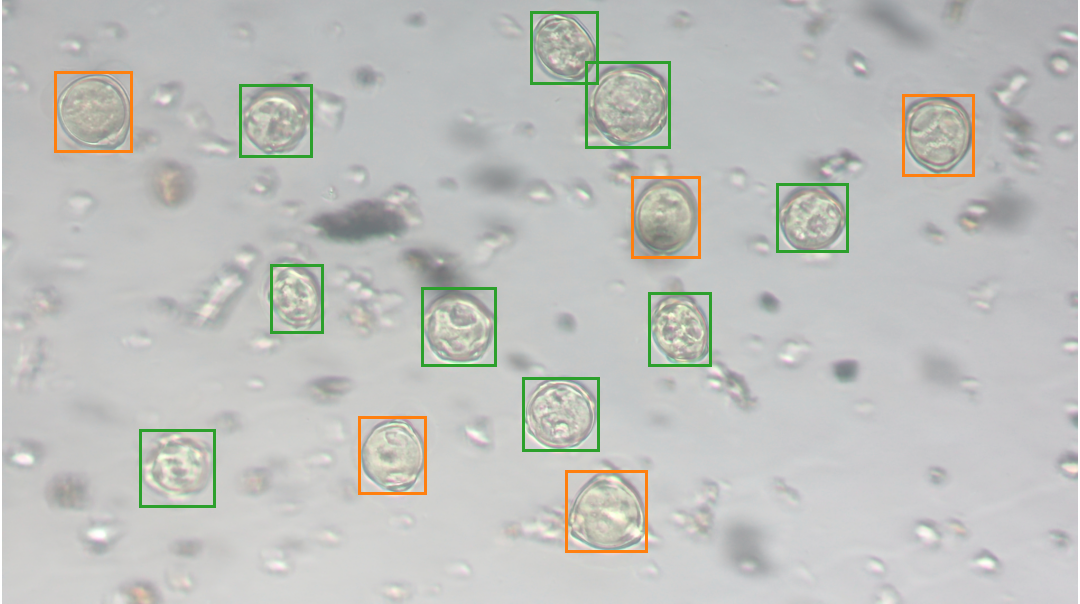
\includegraphics[width=0.8\textwidth]{figs/Snap-057.png}
  \caption[Dataset example]{Example from the dataset with ground truth bounding boxes drawn. The image contains two classes: \textcolor{corylus}{corylus}, and \textcolor{alnus}{alnus}.}\label{fig:dataset-sample}
\end{figure}

Three microscope slides have been imaged using a digital optical microscope producing a set of 701 raster images with a size of \(1080\times 1920\) pixels and three channels; red, green, and blue.
The resolution of each image is \(\SI{0.183}{\micro\metre\per\pixel}\).
Each image has been labeled in collaboration with the experts to produce a valid and correct ground truths.
In total, three different species have been classified, namely \textit{poaceae}, \textit{corylus}, and \textit{alnus}, known in English as Grasses, Hazel, and Alder, respectively. A labeled example is given in Figure~\ref{fig:dataset-sample}. A summary of the dataset is given in Table~\ref{tab:dataset}.

\begin{table}[htb]
  \caption[Class distribution across the dataset]{Distribution of classes across the pollen dataset}\label{tab:dataset}
  \centering 
  \begin{tabular}{lrrr} \toprule
                      & Poaceae & corylus & alnus \\ \midrule
    Number of labels  & 5600    & 262     & 522 \\
    Proportion        & 87.7\%  & 4.1\%   & 8.2\% \\ \bottomrule
  \end{tabular}
\end{table}


Many of the images are taken from the same view point, but with the focus point set to different grains. The ground truth labeled are drawn for all present pollen grains, regardless of the how blurred they appear. This is done so that the dataset may be modified for the purpose of our analysis of sharpness and model performance in regards to \textit{RQ2}.

As opposed to more general object detection tasks, where there is a large variance in both the apparent size and shape of objects within an image, this dataset is much more regular. This is demonstrated in Figure~\ref{fig:aspect}, where we can see that the grains are mostly square in shape and between 100 and 150 pixels wide.

\begin{figure}[htb]
  \centering
  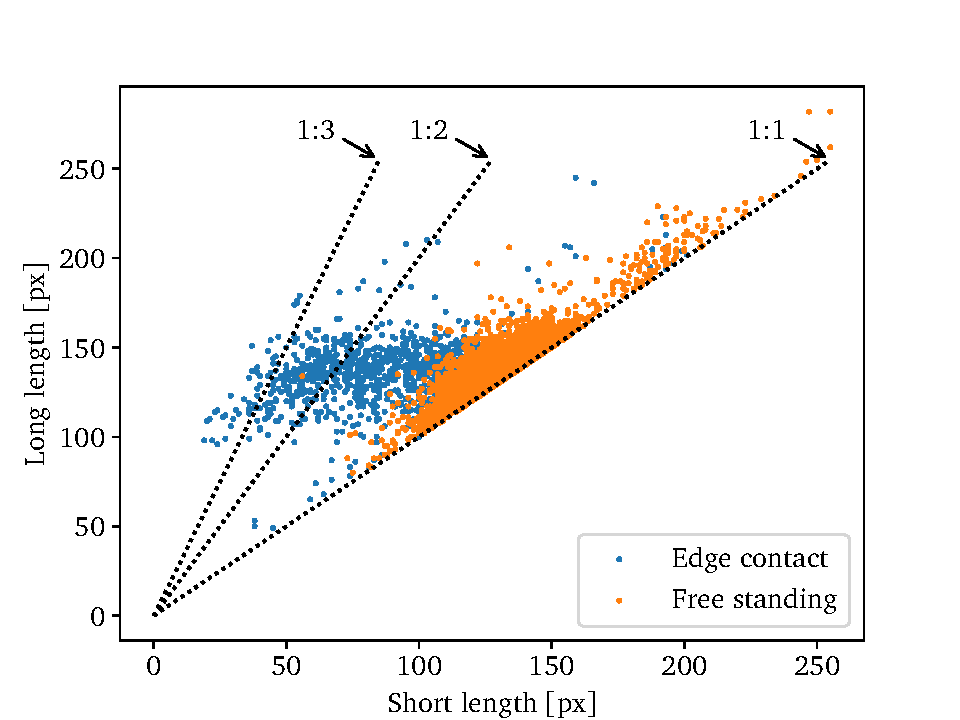
\includegraphics[width=0.9\textwidth]{figs/aspect_ratio.pdf}
  \caption[Aspect ratios in the dataset]{The widths and heights of all ground truth boxes are plotted, longest against shortest. The lines denote the three aspect ratios used in the default boxes of the SSD model. Grains marked `Edge contact' are those in direct contact with the edge of the image and are most likely partially cropped out of frame. We can clearly see that the grains are quite regular in both shape and size}\label{fig:aspect}
\end{figure}

%\section{Architecture}\label{sec:architecture}

\section{Sharpness Measure}\label{sec:method-sharpness}
Analyzing how the sharpness of pollen grains affects detection performance requires an objective sharpness measure.
In this section we will detail how sharpness will be measured for the purpose of our analysis.
The measure is based on Fourier analysis and its performance has been tested on the training data.

\subsection{Fourier analysis}
Fourier analysis describes the general method of utilizing the Fourier transform to analyze the component frequencies present is some signal.
For the purpose of Fourier analysis we can interpret an image as a collection of signals, each of which describe the change in brightness value when traveling across the image in some direction.
Taking the Fourier transform of an image then produces a 2-dimensional matrix where the intensity of each element represents a the coefficient of a 2-dimensional sinusoid base component of the image.
Figure~\ref{fig:fourier-sinusoid} visualizes what the base components look like and demonstrates exactly what is encoded in the Fourier spectrum.

\begin{figure}[htbp]
  \centering
  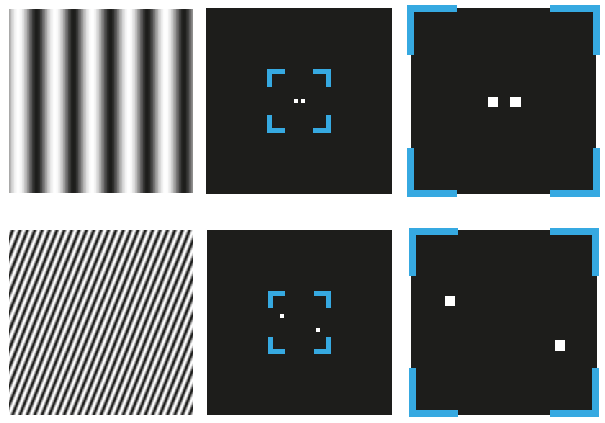
\includegraphics[width=0.8\textwidth]{figs/fourier/fourier-sinusoid.pdf}
  \caption[Fourier transform of sinusoid]{The figure shows two 2D sinusoid wave forms and their Fourier transform. The active components in the transform have been enlarged so as to make them visible in print. Only a single pixel, and its reflection about the origin, is active.}\label{fig:fourier-sinusoid}
\end{figure}

Figure~\ref{fig:fourier-demo} shows the Fourier transform of various inputs.
The transforms are shifted, such that an element in the transform encodes a sinusoid component with a frequency proportional to its distance from the center and moving in the same direction as the vector it forms with the center. 
The directionality of the Fourier transform is demonstrated in the first two examples.
Squares decompose into a set on sinusoids, all moving is the same two directions.
The coefficient of each component is encoded in the intensity of the pixel.
In all the examples the lower frequency components dominate, which lights up the center region. The last two examples demonstrate how blurring an image eliminates the higher frequencies from the Fourier domain.



\begin{figure}[htbp]
  \centering
  \begin{subfigure}[b]{0.2\textwidth}
    \centering
    
\includegraphics[width=\textwidth]{figs/fourier/square_original.png}
    \vspace*{0.02\textwidth}
  \end{subfigure}%
  \hspace*{0.02\textwidth}
  \begin{subfigure}[b]{0.2\textwidth}
    \centering
    
\includegraphics[width=\textwidth]{figs/fourier/square_45deg_original.png}
    \vspace*{0.02\textwidth}
  \end{subfigure}%
  \hspace*{0.02\textwidth}
  \begin{subfigure}[b]{0.2\textwidth}
    \centering
    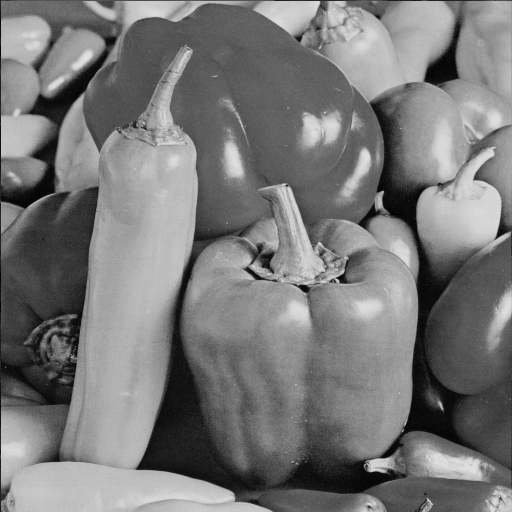
\includegraphics[width=\textwidth]{figs/fourier/peppers_original.png}
    \vspace*{0.02\textwidth}
  \end{subfigure}%
  \hspace*{0.02\textwidth}
  \begin{subfigure}[b]{0.2\textwidth}
    \centering
    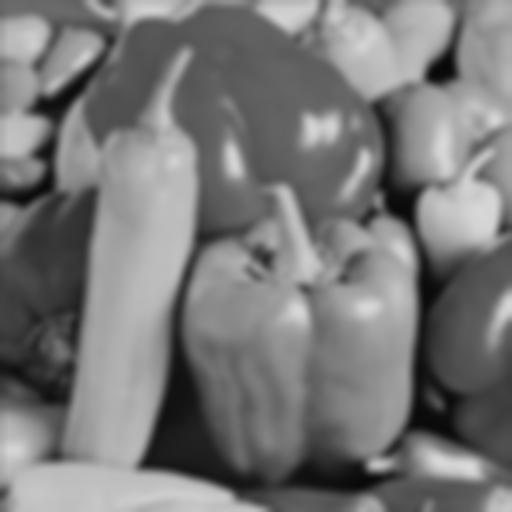
\includegraphics[width=\textwidth]{figs/fourier/peppers_blur_original.png}
    \vspace*{0.02\textwidth}
  \end{subfigure}

  \begin{subfigure}[t]{0.2\textwidth}
    \centering
    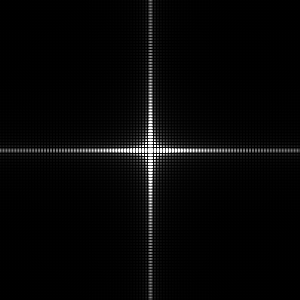
\includegraphics[width=\textwidth]{figs/fourier/square_fourier.png}
  \end{subfigure}%
  \hspace*{0.02\textwidth}
  \begin{subfigure}[t]{0.2\textwidth}
    \centering
    
\includegraphics[width=\textwidth]{figs/fourier/square_45deg_fourier.png}
  \end{subfigure}%
  \hspace*{0.02\textwidth}
  \begin{subfigure}[t]{0.2\textwidth}
    \centering
    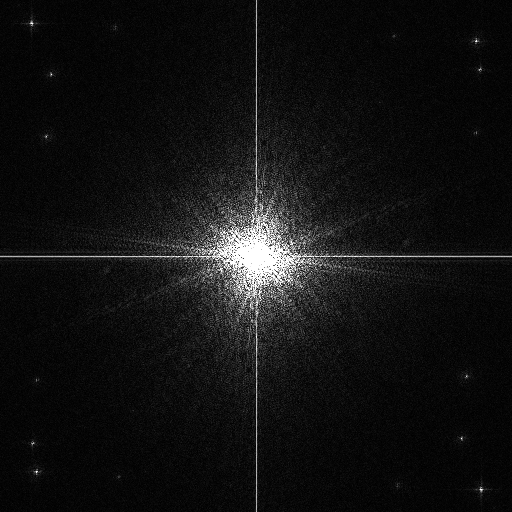
\includegraphics[width=\textwidth]{figs/fourier/peppers_fourier.png}
  \end{subfigure}%
  \hspace*{0.02\textwidth}
  \begin{subfigure}[t]{0.2\textwidth}
    \centering
    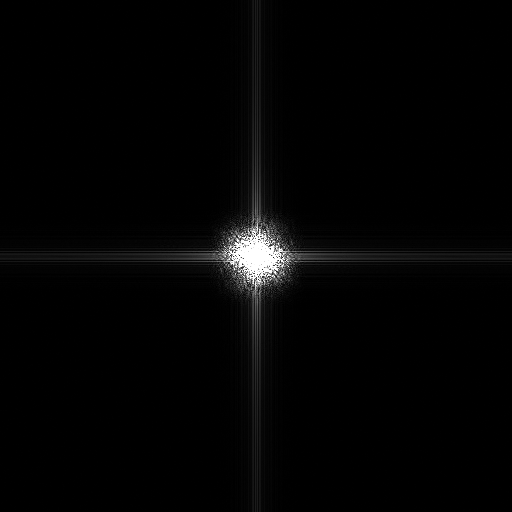
\includegraphics[width=\textwidth]{figs/fourier/peppers_blur_fourier.png}
  \end{subfigure}
  \caption[Demonstration of the Fourier transform]{
    Demonstration of the Fourier transform. The bottom row shows the center-shifted discrete Fourier transform of the corresponding image in the top row. The Fourier spectra mapped to grayscale values with a truncated linear amplitude mapping which is scaled to compensate for the otherwise dominating center component.}\label{fig:fourier-demo}
\end{figure}

Using the Fourier spectrum to measure sharpness follows from the realization that there is a strong relationship between the sharpness of an image in the spacial domain and the distribution of frequency components in the frequency domain.
Sharp features produce high frequencies while blur smooths out the changes in brightness, lowering the frequencies.
Figure~\ref{fig:fourier} shows three different pollen grains, captured with progressively more blur.
If we look at their corresponding Fourier spectra we can see that, as the perceived blur increases, the amount of high frequency components decrease.


\begin{figure}[htbp]
  \centering
  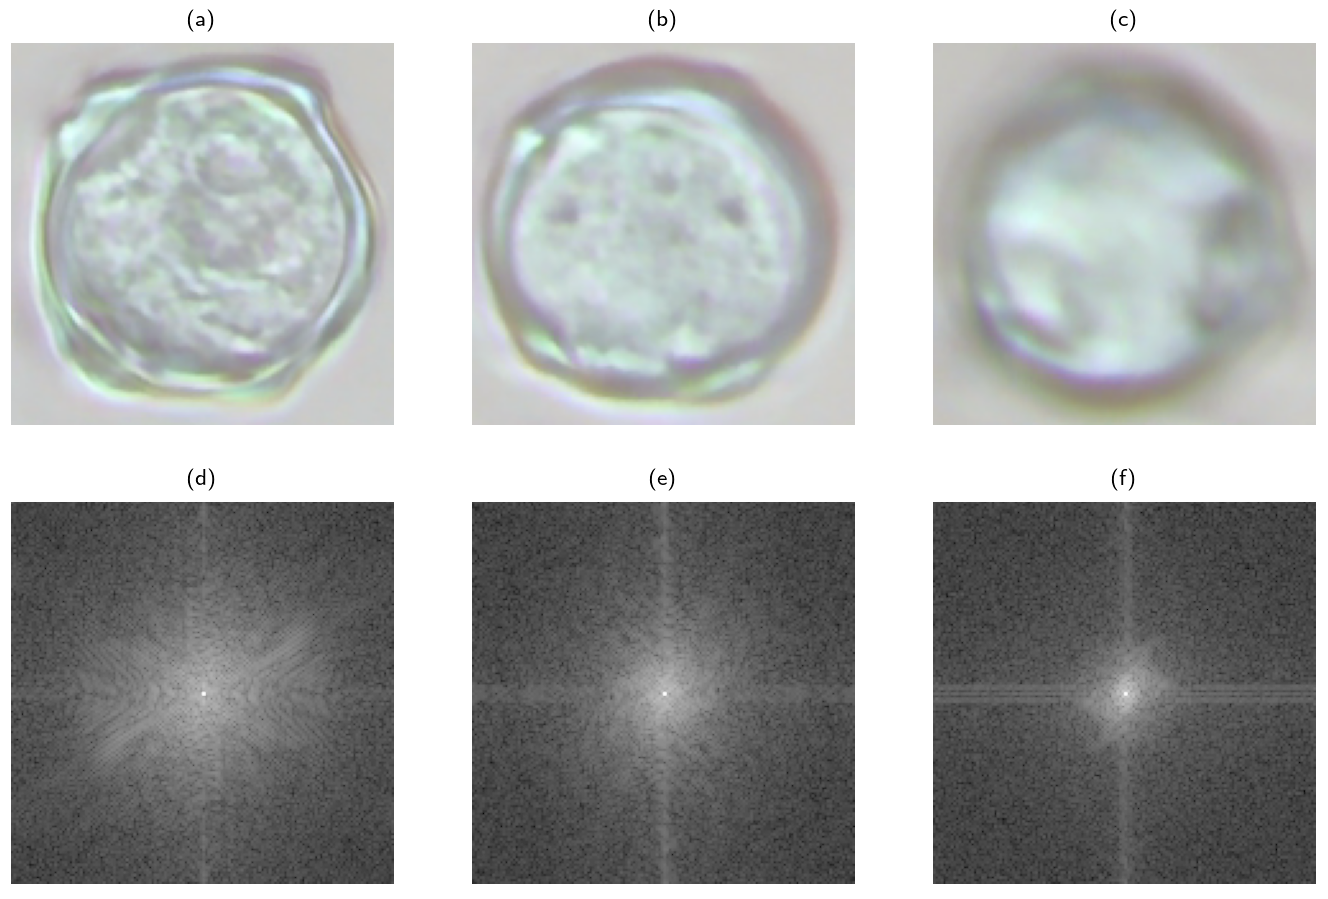
\includegraphics[width=0.8\textwidth]{figs/fourier.png}
  \caption[Fourier spectrum]{Pollen grains and their corresponding centered Fourier spectrum. The Fourier spectra are log scaled so that the higher frequencies become visible.}\label{fig:fourier}
\end{figure}

\subsection{Measuring sharpness}
We must then decide how to encode this change in frequency distribution as a scalar sharpness measure.
\citeauthor{de2013image} propose a simple method which counts the number of components in the Fourier spectrum having a value above a certain threshold.
The operation is described in Equation (\ref{eq:sharp}).


\begin{equation}\label{eq:sharp}
  \begin{split}
    \mathbf{X} &= \mathcal{F}(a),\quad a\in \mathbb{Z}^{M\times N}\\
    T_H &= \sum_{x\in\mathbf{X}}[x\ge\mu],\quad \mu=\frac{\max \mathbf{X^{\mathrm{abs}}}}{1000}\\
    S &= \dfrac{T_H}{M\times N}
  \end{split}
\end{equation}

Here \(\mathcal{F}\) is the discrete the Fourier transform, operating on a input image \(a\), and \(\mathbf{X}\) only contains the magnitude of the Fourier transform.
The scaling factor of the threshold value, \(\mu \), was found to produce good results on our data, without modification. \(S\) is the sharpness measure.

Validating the sharpness measure is an important task.
The weight of any argument made based on analysis using this measure is predicated on its soundness.
There are many different approaches to this, we have chosen to compare the objective measure with subjective measurements of perceived sharpness on a subset of the training data.

\subsection{Evaluating the sharpness measure}
The basis of our evaluation is a new dataset created from a small random subset of the training examples.
Each ground truth is then given sharpness scores based on perceived sharpness and the objective measure.
Determining perceived sharpness of a pollen grain with high fidelity was found to be highly subjective and non-reproducible with repeated independent scoring, so a simple classification was instead performed.
Images where separated into three classes representing perceived sharpness.
Figure~\ref{fig:fourier} gives examples of the classes with image (a) being the sharpest (class 3) and (c) being the blurriest (class 1).
A total of 389 pollen grains where evaluated, the distribution of their classes is given in Table~\ref{tab:sharpness}

\begin{table}[htbp]
  \caption[Sharpness dataset distribution]{Distribution of classes across the sharpness evaluation dataset.}\label{tab:sharpness}
  \centering 
  \begin{tabular}{lrrr} \toprule
    & blurry [1] & partly [2] & sharp [3]  \\ \midrule
    Number of labels & 123 & 105 & 125 \\ \bottomrule
  \end{tabular}
\end{table}

\begin{figure}[htbp]
  \centering
  \begin{subfigure}[t]{0.49\textwidth}
    \centering
    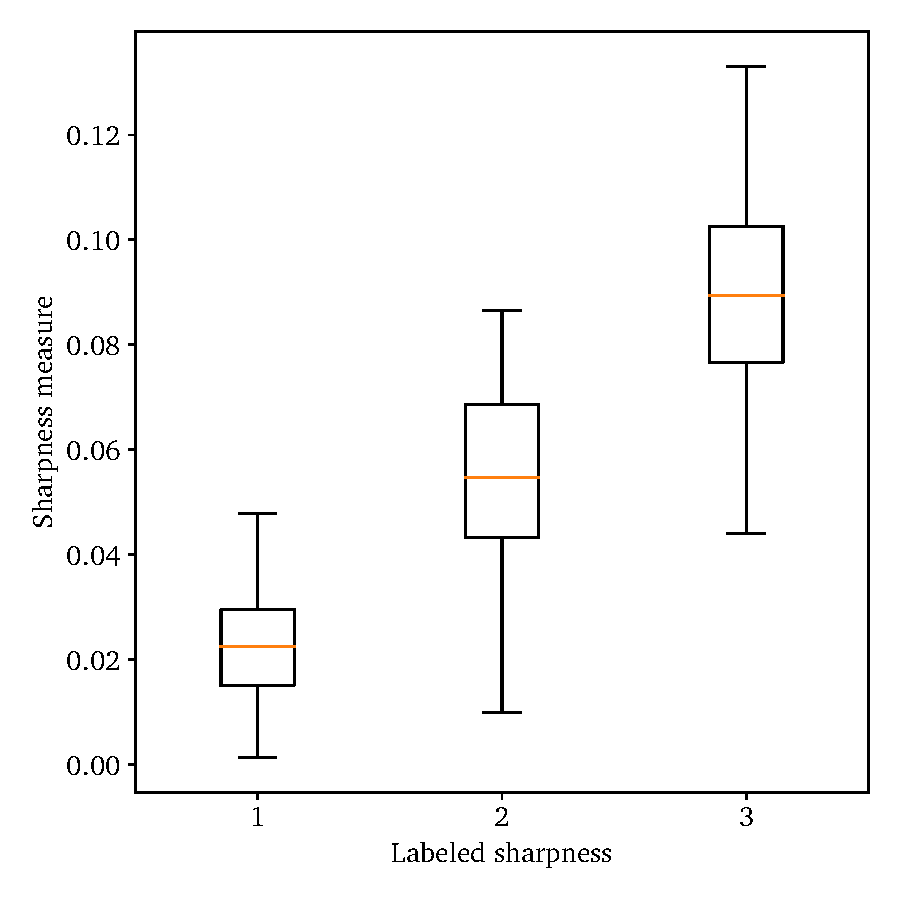
\includegraphics[width=\textwidth]{figs/box.pdf}
    \caption{Box plot}\label{fig:sharpness-box}
\end{subfigure}%
\hfill
\begin{subfigure}[t]{0.48\textwidth}
  \centering
  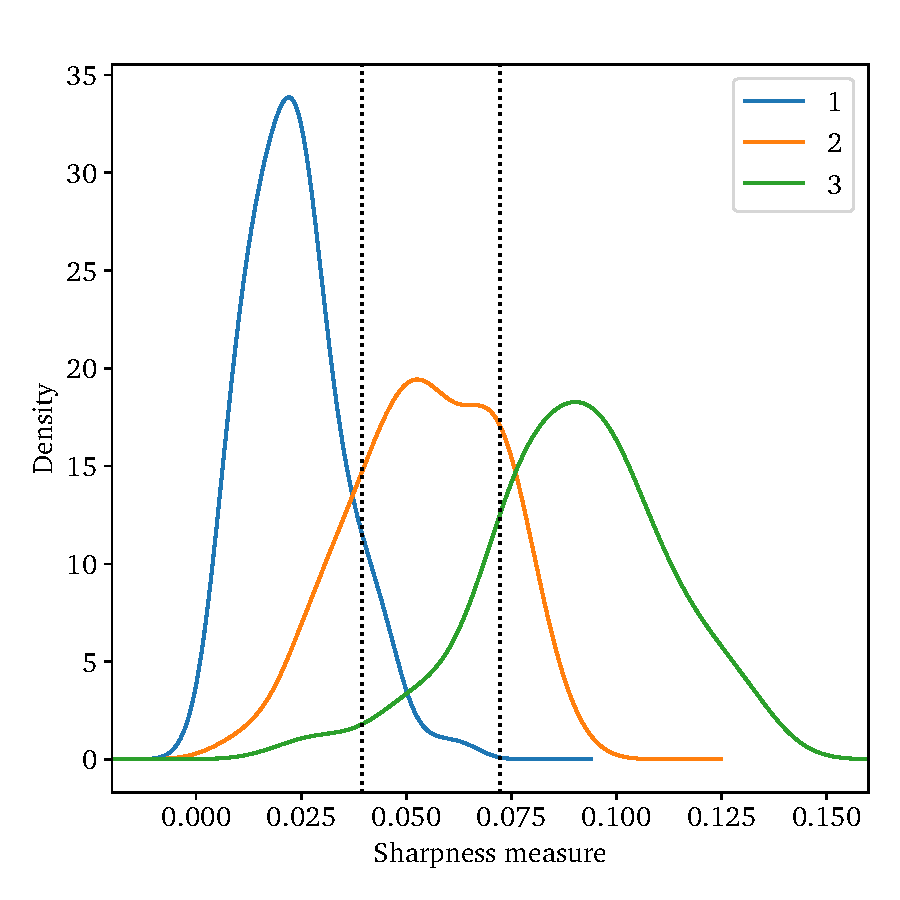
\includegraphics[width=\textwidth]{figs/qden.pdf}
  \caption{Density plot}\label{fig:sharpness-qden}
\end{subfigure}
  \caption[Sharpness measure separability]{The sharpness measure grouped by class label. There is a large overlap between adjacent classes, but the IQRs in (a) are clearly separated. The correlation between perceived and measured sharpness is also clear.}\label{fig:sharpness}
\end{figure}

Looking at Figure~\ref{fig:sharpness} we can see a clear correlation between the mean of the distribution, and the perceived sharpness.
The overlap is to be expected, given the mapping from a continuous predictor onto a categorical label.
To further evaluate the performance of the sharpness measure, we construct a very simple statistical model, in the form of a decision tree, and test its ability to differentiate between the classes.
The model achieved a test accuracy of 84.1\%. 

In Figure~\ref{fig:sharpness-all} we have computed the sharpness of every ground truth in the dataset in a density plot showing the distribution.
As expected, most of the ground truths fall into the sharpest category, but there is a spread, allowing us to analyze the relationship between sharpness and model performance.

\begin{figure}[htbp]
  \centering
  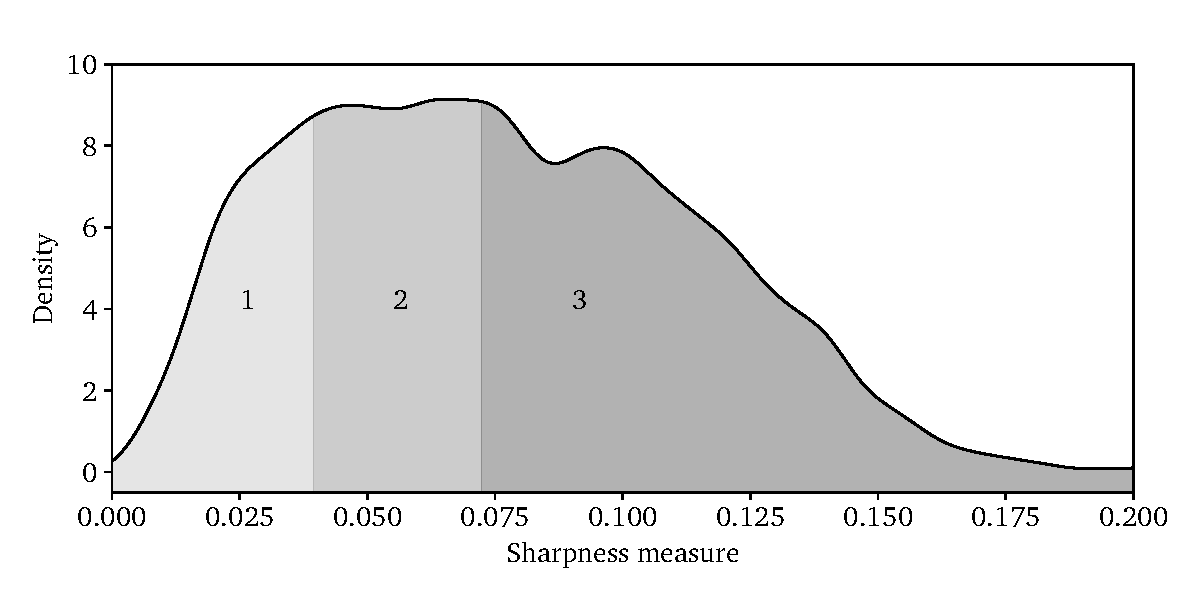
\includegraphics[width=0.9\textwidth]{figs/sharpness_all.pdf}
  \caption[Distribution of sharpness across entire dataset]{Density plot showing the sharpness of all pollen grains in the dataset. The shaded sections indicate the distribution of sharpness classes, if the dataset is classified with the evaluation model. As expected, most grains fall into the sharpest category.}\label{fig:sharpness-all}
\end{figure}